\documentclass{mylib/reporte}
\usepackage{float}

\title{Reporte}
\author{rodrigofranciscopablo }

\subject{Circuitos Eléctricos}
\mytitle{Exposición}
\mysubTitle{Fasores}
\students{
	Avalos Galván María \textsc{Alejandra}\\
	Francisco Pablo \textsc{Rodrigo}\\
	Martínez Pérez \textsc{Oscar}\\
	Peña Salgado \textsc{Gabriel Ulises}
}
\teacher{Ing. Ramírez Hernández \textsc{Benjamin}}
\group{2}
\deliverDate{12 de marzo de 2019}

\begin{document}

\coverPage

\tableofcontents
\newpage

\section{¿Qué es un fasor?}

Un fasor es un número complejo que representa la magnitud y ángulo de fase de un senoide, el ángulo del fasor se basa en el tiempo, puede ser expresado en forma exponencial, polar o rectangular.
En otras palabras y de forma matemática, se denomina fasor a la cantidad compleja .

$$Y=Ye^{j\phi}$$

Cuando un circuito es lineal, las fuentes independientes son senoides y sus frecuencias son constantes se puede representar por medio de fasores, pues permiten simplificar los cálculos, reduciendo un problema de ecuaciones diferenciales a uno algebraico. 

En electricidad, la utilidad de los fasores se deriva de la posibilidad que ofrecen de representar desplazamientos en el tiempo de una señal eléctrica, respecto a una referencia, una dimensión adicional que se añade suponiendo además que los fasores están rotando (se considera que la representación de un diagrama fasorial es como una fotografía en un instante cualquiera de la rotación de los vectores, con el que se puede determinar la diferencia angular entre ellos en ese momento). Se denomina una rotación positiva cuando lo hace en sentido contrario a las agujas del reloj, y negativa cuando rota en el mismo sentido del reloj.

Para describir una señal senoidal de manera de fasor solo se incluye el Vp y el ángulo de desfasamiento.
Los fasores se utilizan generalmente para resolver problemas donde hay que sumar ondas de la misma frecuencia pero de fases y amplitudes distintas para su resolución se dibuja un fasor para cada onda y se aplica una suma vectorial.

\begin{figure}[H]
	\centering
	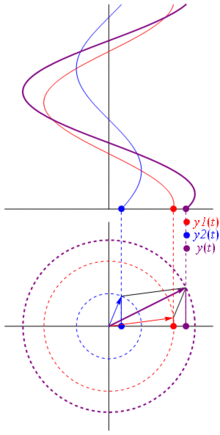
\includegraphics[scale=0.5]{img/circ_expo/image7}
	\caption{Tres fasores moviendose en el dominio de la frecuencia.}
\end{figure}

Podemos usar fasores en voltaje, corriente y resistencia, y por ellos también nos sirve para resolver circuitos con capacitores e inductores, con los valores de su impedancia pero colocados como número imaginario.

Debido a las propiedades de la matemática de oscilaciones, en electrónica los fasores se utilizan habitualmente en el análisis rudimentario de circuitos en AC. Finalmente, los fasores pueden ser utilizados para describir el movimiento de un oscilador. Las proyecciones del fasor en los ejes x e y tiene diferentes significados físicos.

Los fasores son particularmente útiles cuando aplicamos un voltaje de amplitud fija que varía sinusoidalmente en el tiempo y además lo hace a una frecuencia fija. En este caso hablamos de “Régimen Sinusoidal Permanente” (RSP), es decir, la aplicación de una señal de voltaje sinusoidal a un circuito durante un período que se prolonga más allá de su respuesta transitoria. 

\begin{figure}[H]
	\centering
	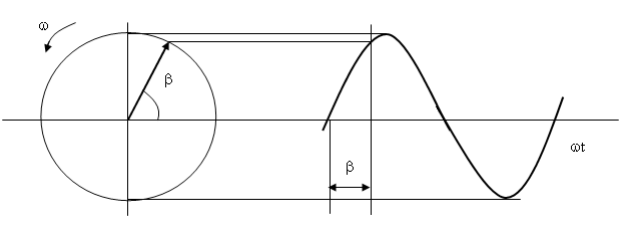
\includegraphics[scale=0.5]{img/circ_expo/image4}
	\caption{A medida que el fasor va rotando se obtiene una función seno o coseno.}
\end{figure}

En este gráfico se puede apreciar que, mientras el fasor gira los 360 grados del diagrama la señal sinusoidal va recorriendo su rango de valores, de forma tal que cuando el fasor completa un giro, también se completa el período de la señal. Esta es la base de la representación que nos facilita el diagrama fasorial, la rotación del vector representa el valor de la función en el tiempo. En un mismo diagrama se pueden representar simultáneamente los voltajes y las corrientes en varios elementos de un circuito, de acuerdo con la respuesta que tenga cada uno.

\section{Diagrama Fasorial}

Diagrama en el que se representan los fasores correspondientes de las tensiones y  corrientes de un circuito en el plano complejo.

\begin{figure}[H]
	\centering
	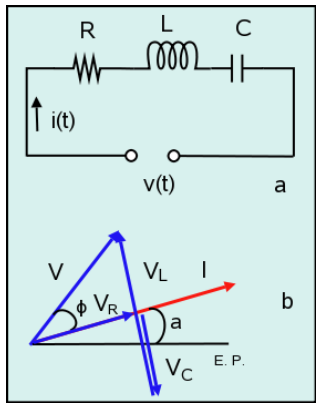
\includegraphics[scale=0.5]{img/circ_expo/image9}
	\caption{Representación que gráfica de los fasores que equivalen al circuito mostrado arriba.}
\end{figure}

\section{Triángulo de impedancias}

El triángulo de impedancia de un elemento o de un circuito se forma representando a la parte real de la impedancia (correspondiente a la resistencia) y a la parte imaginaria (correspondiente a la diferencia entra las reactancias inductiva y capacitiva) en los catetos de un triángulo.

La hipotenusa se calcula de la misma forma que el módulo de un número complejo, es decir mediante el teorema de Pitágoras.

\begin{figure}[H]
	\centering
	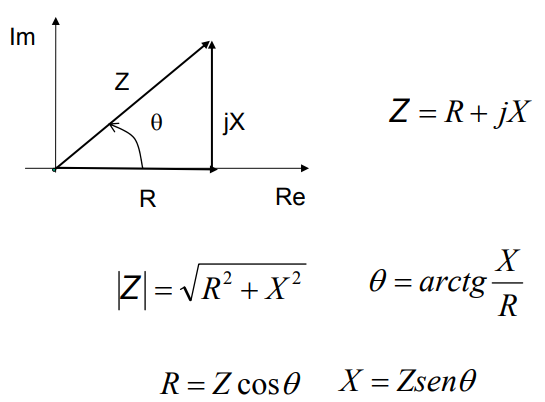
\includegraphics[scale=0.4	]{img/circ_expo/image3}
	\caption{Ejemplo de in triángulo de impedancias.}
\end{figure}

\section{Diagrama fasorial circuito RLC serie}

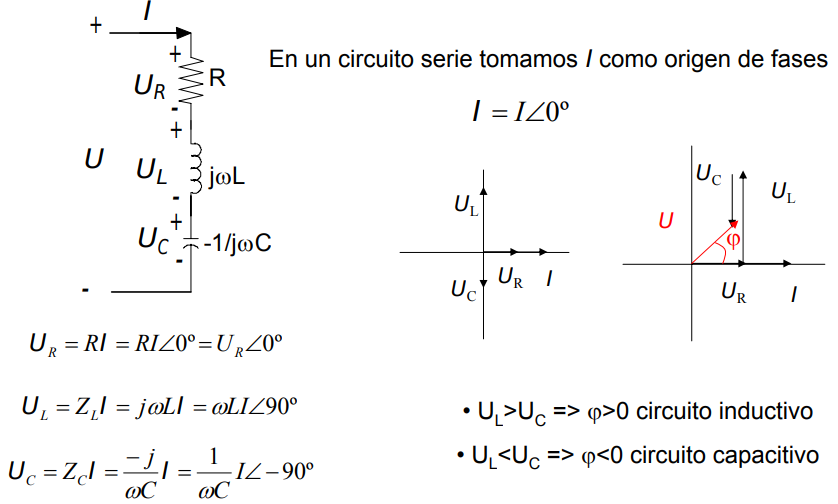
\includegraphics[scale=0.5]{img/circ_expo/image2}

\section{Diagrama fasorial circuito RLC paralelo}

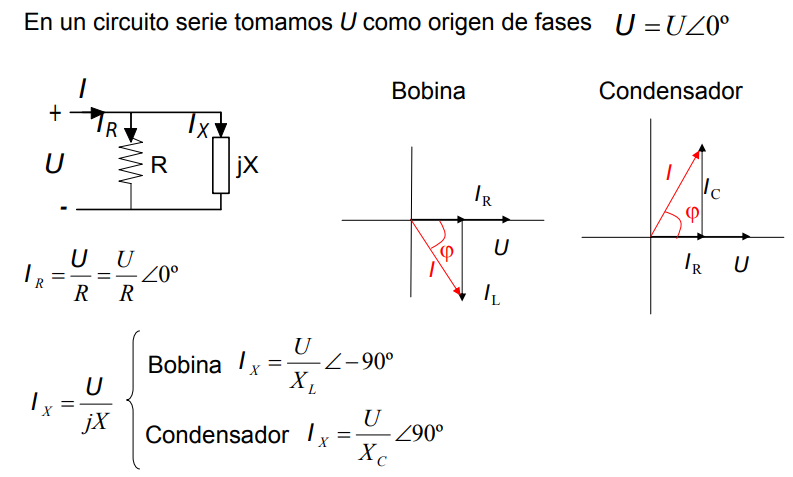
\includegraphics[scale=0.5]{img/circ_expo/image1}

\section{Respuesta en estado senoidal permanente empleando fasores}

En la siguiente tabla se presentan las ecuaciones fasoriales de las fuentes, resistor, inductor y capacitor, el voltaje y corriente fasoriales se presentan relacionados mutuamente.

\begin{figure}[H]
	\centering
	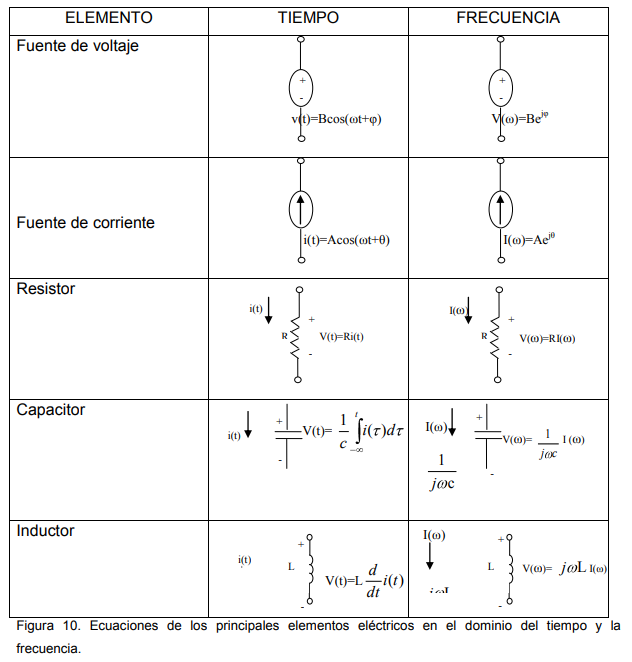
\includegraphics[scale=0.4]{img/circ_expo/image8}
\end{figure}

\section{Bibliografia}

\begin{itemize}
	\item https://prezi.com/ylqprxartrfv/que-es-fasor-para-que-nos-sirve/
	\item https://es.wikipedia.org/wiki/Fasor
	\item http://www.ptolomeo.unam.mx:8080/xmlui/bitstream/handle/\\
		132.248.52.100/941/Tesis.pdf?sequence

\end{itemize}

\section{Liga de descarga}

Para obtener la presentación debe ingresar a http://bit.ly/fasores-cir2019-2

\end{document}
